\documentclass{bioinfo}

\usepackage{subfigure}

\copyrightyear{2010}
\pubyear{2010}

\begin{document}
\begin{application}
\firstpage{1}

\title[SMM Project]{Stabilization matrix method - Mini project}
\author[Sigmar Stef\`{a}nsson, Francesco Favero]{Sigmar Stef\`{a}nsson and Francesco Favero}

\address{Danmarks Tekniske Univeristet}

\history{2 December 2010}

\editor{Supervisor: Morten Nielsen}

\maketitle

\begin{abstract}

   % Abstract
%\section{Summary}


The identification of MHC binding peptides for consideration as potential T-cell epitopes has application in peptide vaccine design and immunotherapy. 
Determination of MHC binding using experimental measures is time-consuming and expensive. 
Therefore, efficient prediction models are required that facilitate systematic computational scanning of microbial genome for candidate T cell epitopes. 
These prediction models are either sequence or structure based. 
This review provides a comparative analysis on machine learing methods support vector machine (SVM) and artificial neural networks (ANN).

\end{abstract}

\section*{Introduction}
   % Introduction

It took more than 20 years for scientist to understand the  physiological role of MHC molecules in peptide presentation to T lymphocytes. 
MHC molecules were initially defined as antigens that stimulate an organism’s immunologic response to transplanted organs and tissues. MHC proteins are found in all higher vertebrates. 
In humans they are called Human Leukocyte Antigens (HLA).

There are two main classes of MHC molecules. Class I and Class II. The genes which encode the various polypeptides forming the two classes of MHC are placed in the genome in the same chromosome.
Two different clusters encode the two different MHC classes. This means that all the genes encoding the class I MHC molecules (HLA-A, HLA-B and HLA-C) are neighbours in a region of chromosome 6,
while the genes encoding the class II MHC molecules (HLA-DP, HLA-DQ and HLA-DR) are close to each other in another region of the same chromosome.

One of the features of MHC is the exceptional allelic diversity. HLA-A and HLA-B have roughly 1000 and 1600 alleles respectively. 
The evolutionary reason for this diversity would be the benefit in the defence of pathogens. 
There is less than 1\% chance that a MHC molecule presents a peptide and different hosts sample different peptides from same pathogen. 
The more diverse MHC molecule the more diversity in presented peptides. As few humans share the same set of HLA alleles, different persons react differently to a pathogen infection. 
This increases the likelihood that at least some individuals of a population will survive an epidemic.

Class-I molecules are present in every cell but Class-II are found on certain immune cells, like macrophages and B-cells. 
These so called antigen-presenting cells (APCs) ingest microbes, destroy them, and digest them into fragments, which are in turn presented by the MHC molecules on the surface of the cell.

The MHC proteins serve to alert the immune system if a foreign material is present inside a cell.
They achieve this by displaying fragmented pieces of antigens on the host cell surface. These antigens can be self or non-self. 
If a host cell was infected by a bacterium or virus, or was cancerous, it may  display the antigens on its surface.
Cells constantly process endogenous proteins and present them within the context of MHC Class-I. 
Immune effector cells are trained not to react to self peptides during a complex process taking place in the thymus.

Only certain types of peptides bind to certain types of MHC molecules. Most peptides selected by class-I molecules are 8 to 10 residues long
and somewhat longer for class-II molecules. The antigenic peptide is located in a cleft existing between the $\alpha_1$ and $\alpha_2$ regions in the heavy chain of the MHC protein.

A CTL based vaccine must include epitopes specific to each HLA allele in a population, also it must deal with pathogen diversity. As result a vaccine must consist of around 1000 HLA class I epitopes.
Less than 70 HLA alleles have been characterized by binding data. Apart from predicting peptide binders in a protein sequence, it is still  mostly unsolved task of how to select the immunogenic proteins in large pathogens.

The classification of MHC peptide binding is a complex task as the mechanics of binding are not fully understood. 
This makes the problem an ideal task for machine learning methods. We compare binding data classification results from PSSM and the machine learning methods support vector machines (SVM) and artificial neural networks (ANN).

Using amino acid properties such as hydropathy index, side-chain polarity or charge and isoelectric point are not sufficient for classification although they can give clues on which locations on the peptide are more important to successful binding than others. 
Some of these properties are taken into account in the z-score amino acid encoding scheme. Structural properties of the MHC molecule are also important in governing the binding affinity.

Some efforts are being made using molecular dynamics simulation and crystal structure data for MHC peptide binding predictions, although these have not proved successful compared to the sequence based methods.

All of the software tools used in this investigation are part of the course and available at CBS apart from the Weka software we used for the SVM calculations. [reference: http://www.cs.waikato.ac.nz/~ml/weka/]

It took 20 years for scientist to understand the  physiological role of MHC molecules in peptide presentation to T lymochytes. 
MHC molecules were initially defined as antigens that stimulate an organism’s immunologic response to transplanted organs and tissues. MHC proteins are found in all higher vertebrates. 
In humans the MHC molecules are called Human Leukocyte Antigens (HLA).
There are two classes of MHC molecules. Each human cell expresses 6 MHC class-I alleles or one HLA-A, B and C allele from each progenitor and 6-8 class-II alleles.
One of the features of MHC is the exceptional allelic diversity. HLA-A and HLA-B have roughly 1000 and 1600 alleles respectively. 
The most obvious evolutionary reason for this would be the benefit of diversity in defence of pathogens. 
There is less than 1% chance that a MHC molecule presents a peptide and different hosts sample different peptides from same pathogen. 
The more diverse MHC molecule the more diversity in presented peptides. As few humans share the same set of HLA alleles, different persons react differently to a pathogen infection. 
This increases the likelihood that at least some individuals of a population will survive an epidemic.
Class-I molecules are present in every cell but Class-II are found on certain immune cells, like macrophages and B-cells. 
These so called antigen-presenting cells (APCs) ingest microbes, destroy them, and digest them into fragments, which are in turn presented by the MHC molecules on the surface of the cell.
The MHC proteins serve to alert the immune system if foreign material is present inside a cell. 
They achieve this by displaying fragmented pieces of anigens on the host cell surface. These antigens can be self or non-self. 
If a host cell was infected by a bacterium or virus, or wascancerous, it may  display the antigens on its surface.
Cells constantly process endogenous proteins and present them within the context of MHC Class-I. 
Immune effector cells are trained not to react to self peptides during a complex process taking place in the thymus.
Only certain types of peptides bind to certain types of MHC molecules. Most peptides selected by class-I molecules are 8 to 10 residues long. 
Somewhat longer for class-II molecules. The antigenic peptide is located in a cleft existing between the α1 and α2 regions in the heavy chain of the MHC protein.
A CTL based vaccine must include epitopes specific to each HLA allele in a population. Also it must deal with pathogen diversity, e.g. it must consist of around 1000 HLA class I epitopes. 
Less than 70 HLA alleles have been characterized by binding data. Apart from predicting peptide binders in a protein sequence, it is still  mostly unsolved task of how to select the immunognic proteins in large pathogens.
The classification of MHC peptide binding is a highly complex task as the mechanics of binding are not fully understood. 
This makes the problem an ideal task for machine learning methods. We compare binding data classification results from PSSM and the machine learing methods support vector machines (SVM) and artifical neural networks (ANN).
Using amino acid properties such as hydropathy index, side-chain polarity or charge and isoelectric point is not sufficient for classification although they can give clues on which locations on the peptide are more important to succesful binding than others. 
Structural properties of the MHC molecule are therefore important in governing the binding affinity.
Some efforts are being made using molecular dynamics simulation and crystal structure data with no experimental data for training, although these have not proved succesful.

\section*{Material and Methods}
   %Material and Methods

In all cases the Pearson's correlation coefficient was used to evaluate and compare the predictive performance the the three methods, PSSM\cite{PSSM}, SVM\cite{SVM} and ANN\cite{ANNf}\cite{ANNb}

\begin{table}[ht]\scriptsize
\begin{center}
\begin{tabular}{rllrrr}
\hline
 & Allele	&	 binders & total & \% of binders \\
\hline
 & A2402	&	99	&	197	&	50\%	\\
 & A2301	&	49	&	104	&	47\%	\\
 & A0202	&	649	&	1447	&	45\%	\\
 & A0203	&	639	&	1443	&	44\%	\\
 & A6801	&	498	&	1141	&	44\%	\\
 & B4501	&	49	&	114	&	43\%	\\
 & A2902	&	68	&	160	&	43\%	\\
 & B5301	&	106	&	254	&	42\%	\\
 & B1801	&	47	&	118	&	40\%	\\
 & A0201	&	1181	&	3089	&	38\%	\\
 & B4402	&	44	&	119	&	37\%	\\
 & A0206	&	513	&	1437	&	36\%	\\
 & A1101	&	693	&	1985	&	35\%	\\
 & B5101	&	85	&	244	&	35\%	\\
 & B4002	&	39	&	118	&	33\%	\\
 & B5401	&	81	&	255	&	32\%	\\
 & A3002	&	29	&	92	&	32\%	\\
 & B3501	&	211	&	736	&	29\%	\\
 & B4403	&	34	&	119	&	29\%	\\
 & A6802	&	397	&	1434	&	28\%	\\
 & A0301	&	517	&	2094	&	25\%	\\
 & A3101	&	427	&	1869	&	23\%	\\
 & B5701	&	11	&	59	&	19\%	\\
 & B1501	&	179	&	978	&	18\%	\\
 & B0702	&	208	&	1262	&	16\%	\\
 & A3301	&	184	&	1140	&	16\%	\\
 & A3001	&	77	&	669	&	12\%	\\
 & A2403	&	29	&	254	&	11\%	\\
 & B5801	&	104	&	988	&	11\%	\\
 & A6901	&	86	&	833	&	10\%	\\
 & A0101	&	103	&	1157	&	9\%	\\
 & A2601	&	53	&	672	&	8\%	\\
 & B2705	&	56	&	969	&	6\%	\\
 & B4001	&	40	&	1078	&	4\%	\\
 & B0801	&	20	&	708	&	3\%	\\
\hline
\end{tabular}
\caption{Content of bindings and not bindings peptides for each allele dataset. The samples are in decreasing order of the percentage of binding peptides.}\label{ftable}
\end{center}
\end{table}



\subsection*{PSSM}
A Position-specific scoring matrix, also called position weight matrix is a commonly used representation of motifs in biological sequences. 
It has one row for each symbol in the alphabet (amino acid, for instance) and one column for each position in the motif.
The weight matrix is constructed using log-odds score

\begin{equation}
W_{ij} = \log{ (\frac{p_{ij}}{q_j}) }
\end{equation}

i being the position in the motif and j the amino acid. $q_j$ is the background frequency for ammino acid j. 
The score of a sequence is simply the sum of the position-specific scores for each symbol in the substring.

\begin{equation}
s = \sum_{i}{W_{i}} \\
\end{equation}

where j represents position in the substring, i is the symbol at position j in the substring and $W_{i}$ is the corresponding score in the weight matrix.

PSSM scores can be interpreted as the sum of binding energies for all nucleotides or amino acids aligned with the PSSM and can as such be used to estimate MHC peptide binding affinity.

Sequence weighting can be used to reduce redundancy and emphasize diversity. In the case of MHC peptide binding it is used to compensate for poor or biased sampling of sequence space.
Simply put, the weight on a peptide k at position p is

\begin{equation}
w_{kp} = \frac{1}{r\cdot s}
\end{equation}

where r is the number of different amino acids in the column p, and s is the number of occurrence of amino acids a in that column. The weight of the sequence k is then the sum of the weights over all positions

\begin{equation}
w_{k} = \sum_{p}{\frac{1}{r_p \cdot s_p}}
\end{equation}

Pseudo count is used to compensate for few data points and is estimated as

\begin{equation}
g_b = \sum{f_a}{q_{b|a}}
\end{equation}

where $f_a$ is the observed amino acid frequency. The $q_{a|b}$ is the probability of amino acid b given amino acid a and is acquired from a Blosum substitution frequency matrix.
The Blosum substitution matrix, is a
conditional probability matrix of matching amino
acids j given you have amino acid i

\begin{equation}
P(j|i) = \frac{P_ij}{Q_i}
\end{equation}

the matrix is used to for the pseudo count in creation of the PSSM matrix. 

Pseudo counts are important when only limited data is available. With large datasets only the observation should count:

\begin{equation}
p_a = \frac{\alpha \cdot f_a + \beta \cdot g_a}{\alpha + \beta}
\end{equation}

$\alpha$ is the effective number of sequences and $\beta$ is the weight on prior and concerns the size of the data set when pseudo count are taken into account.

The information content of a position in a peptide an indicator of how different its distribution is from a uniform distribution and is calculated using Shannon's discrete entropy law (the sum part of the equation \ref{info})

\begin{equation}
\label{info}
I = \log{ 20 } + \sum_{a}{ p_{a}\log{p_{a}} }
\end{equation}

where $p_a$ is the probability of the symbol a in sequence (for some position in the peptide). The information content is used to estimate which positions in a peptide are more important to the MHC binding than others 
(and to construct so called sequence logos).

\subsection*{SVM}
Support vector machines is a set of supervised learning methods used for classification and regression analysis. 
The standard SVM is non-probabilistic binary linear classifier. 
It constructs a hyperplane where the separation is where there is largest distance to the nearest training data point of any class. 
Non-linear classification can be achieved by  mapping the original space to a higher dimensional feature space and/or select a kernel function to suit the problem. 
The kernel function then plays the role of the dot product in the feature space.

In the linear SVM we want to find the maximum-margin hyperplane that divides the points having (class) $y_{i}$ = 1 from those having $y_i = -1$. Any hyperplane can be written as the set of points \b{x} satisfying

\begin{equation}
\mathbf{w \cdot x} - b = 0
\end{equation}

We want to choose the \b{w} and b to maximize the margin, or distance between the parallel hyperplanes that are as far apart as possible while still separating the data. These hyperplanes can be described by the equations

\begin{equation}
\mathbf{w \cdot x} - b = 1
\end{equation}

and

\begin{equation}
\mathbf{w \cdot x} - b = -1
\end{equation}

The distance between these two hyperplanes is $\frac{2}{||w||}$, so we wan't to minimize $||w||$.
To prevent data points falling into the margin, we add the following constraint:

\begin{equation}
y_i(\mathbf{w \cdot x} - b) \geq 1, for all 1 \leq i \leq n
\end{equation}

where $y_i$ is the class point i belongs to.

Substituting $||w||$ with $\frac{1}{2}||w||^2$ makes this a quadratic optimization problem. 
The solution involves constructing a dual problem where 
a Lagrange multiplier $\alpha_i$ 
is associated with every 
constraint in the primary problem. Mathematically put, find $\alpha_1 \cdots \alpha_n$
such that

\begin{equation}
\mathbf{Q(\alpha)} = \sum_{i=1}^{n}{\alpha_i} - \frac{1}{2}\sum_{i,j}{\alpha_i\alpha_j y_i y_j \mathbf{x_i^T x_j} }
\end{equation}

is maximized knowing $\mathbf{w} = \sum_{i}{ \alpha_i y_i \mathbf{x_i} }$ and $\sum_{i}{\alpha_i y_i} = 0$ and $\alpha_i \geq 0$ for all $\alpha_i$.  
A common method for solving the QP problem is the Sequential Minimal Optimization (SMO) algorithm, 
which breaks the problem down into 2-dimensional sub-problems that may be solved analytically, eliminating the need for a numerical optimization algorithm.
We choose the SMO method for classification in the Weka software.

\subsection*{ANN}
Artificial neural networks are used to model complex relationships between inputs and outputs or to find patterns in data.
Neural networks are non-linear statistical data modelling tools, in most cases an adaptive system that changes its structure based on external or internal information that flows through the network during the learning phase.
The effect on the binding affinity of
having a given amino acid at one
position can be influenced by the
amino acids at other positions in the
peptide. Artificial neural networks are
ideal to take such
correlations into account. Similar to equation \ref{info} a mutual information is defined as

\begin{equation}
\label{mutinfo}
I = \sum_{a,b}{ p_{ab}\log{ \frac{ p_{ab} }{ p_a \cdot p_b } } }
\end{equation}

where $p_{ab}$ is the probability of having amino acids of type a and b in certain positions of the peptide. $p_a$ and $p_b$ are the probabilities of having the corresponding amino acids in the relevant positions in the peptide.
Having sequence correlations demands the classifier to be able to do model a non-linear function (XOR function). Neural network achieve this by adding a hidden layer/neurons.

Associated with every edge of the neural network graph is a weight $w_i$, so the output becomes:

\begin{equation}
o = \sum{x_i \cdot w_i}
\end{equation}

The sigmoid function is used for the output of each neuron:

\begin{equation}
O = \frac{1}{1+\exp{(-o)}}
\end{equation}

The adaptation in the network is achieved by minimizing error by varying the weights. The quadratic error is defined as:

\begin{equation}
E = \frac{1}{2}\sum_{\alpha i}{(O_i^\alpha - T_i^\alpha)^2}
\end{equation}

Then the weights are varied for example with the gradient descent method

\begin{equation}
\Delta w = -\epsilon \frac{\delta E}{\delta w}
\end{equation}

\subsection*{Overfitting}
Overfitting\cite{wiki:overfit} occurs when a statistical model describes random error or noise instead of the underlying relationship.
This can happen when a model is excessively complex, such as having too many parameters relative to the number of observations.
To prevent overfitting a cross-validated training is used. 1/5 of the data is used for testing and 4/5 for training. 
The training is stopped when the test performance is optimal. This is done for each of the 5 sections of the data and the result is 5 different sets of network weights/synapses.
The synapses are then used when evaluating the network.
Optimally one would take one part of the data aside for final evaluation of the network. This part would be used in neither the training nor the testing.
We wanted to have as large sets of peptide data as possible. 
For the smaller datasets we made a cross-validated training/testing on the whole dataset and then evaluated with testing data using synapses not created with that testing dataset.
As a result the networks for the smaller datasets are possibly slightly overfit (e.g. evaluation data is also in the the training data).
For the larger datasets, we also took 1/5 of the data aside for the evaluation and did a 4-fold cross-validation on the remaining 4 parts.

\subsection*{Data}
We mostly used peptide binding data from class-I MHC molecules (A and B types) as they were readily available to us.
To get a better grasp on the the expected quality of the results in the machine learning methods we did evaluate the fraction between binding and non-binding peptides in the dataset for each data {\ref{ftable}}

In the PSSM case only the binders are used, so datasets with few of them could give bad results.

\begin{figure*}[ht]
\begin{center}
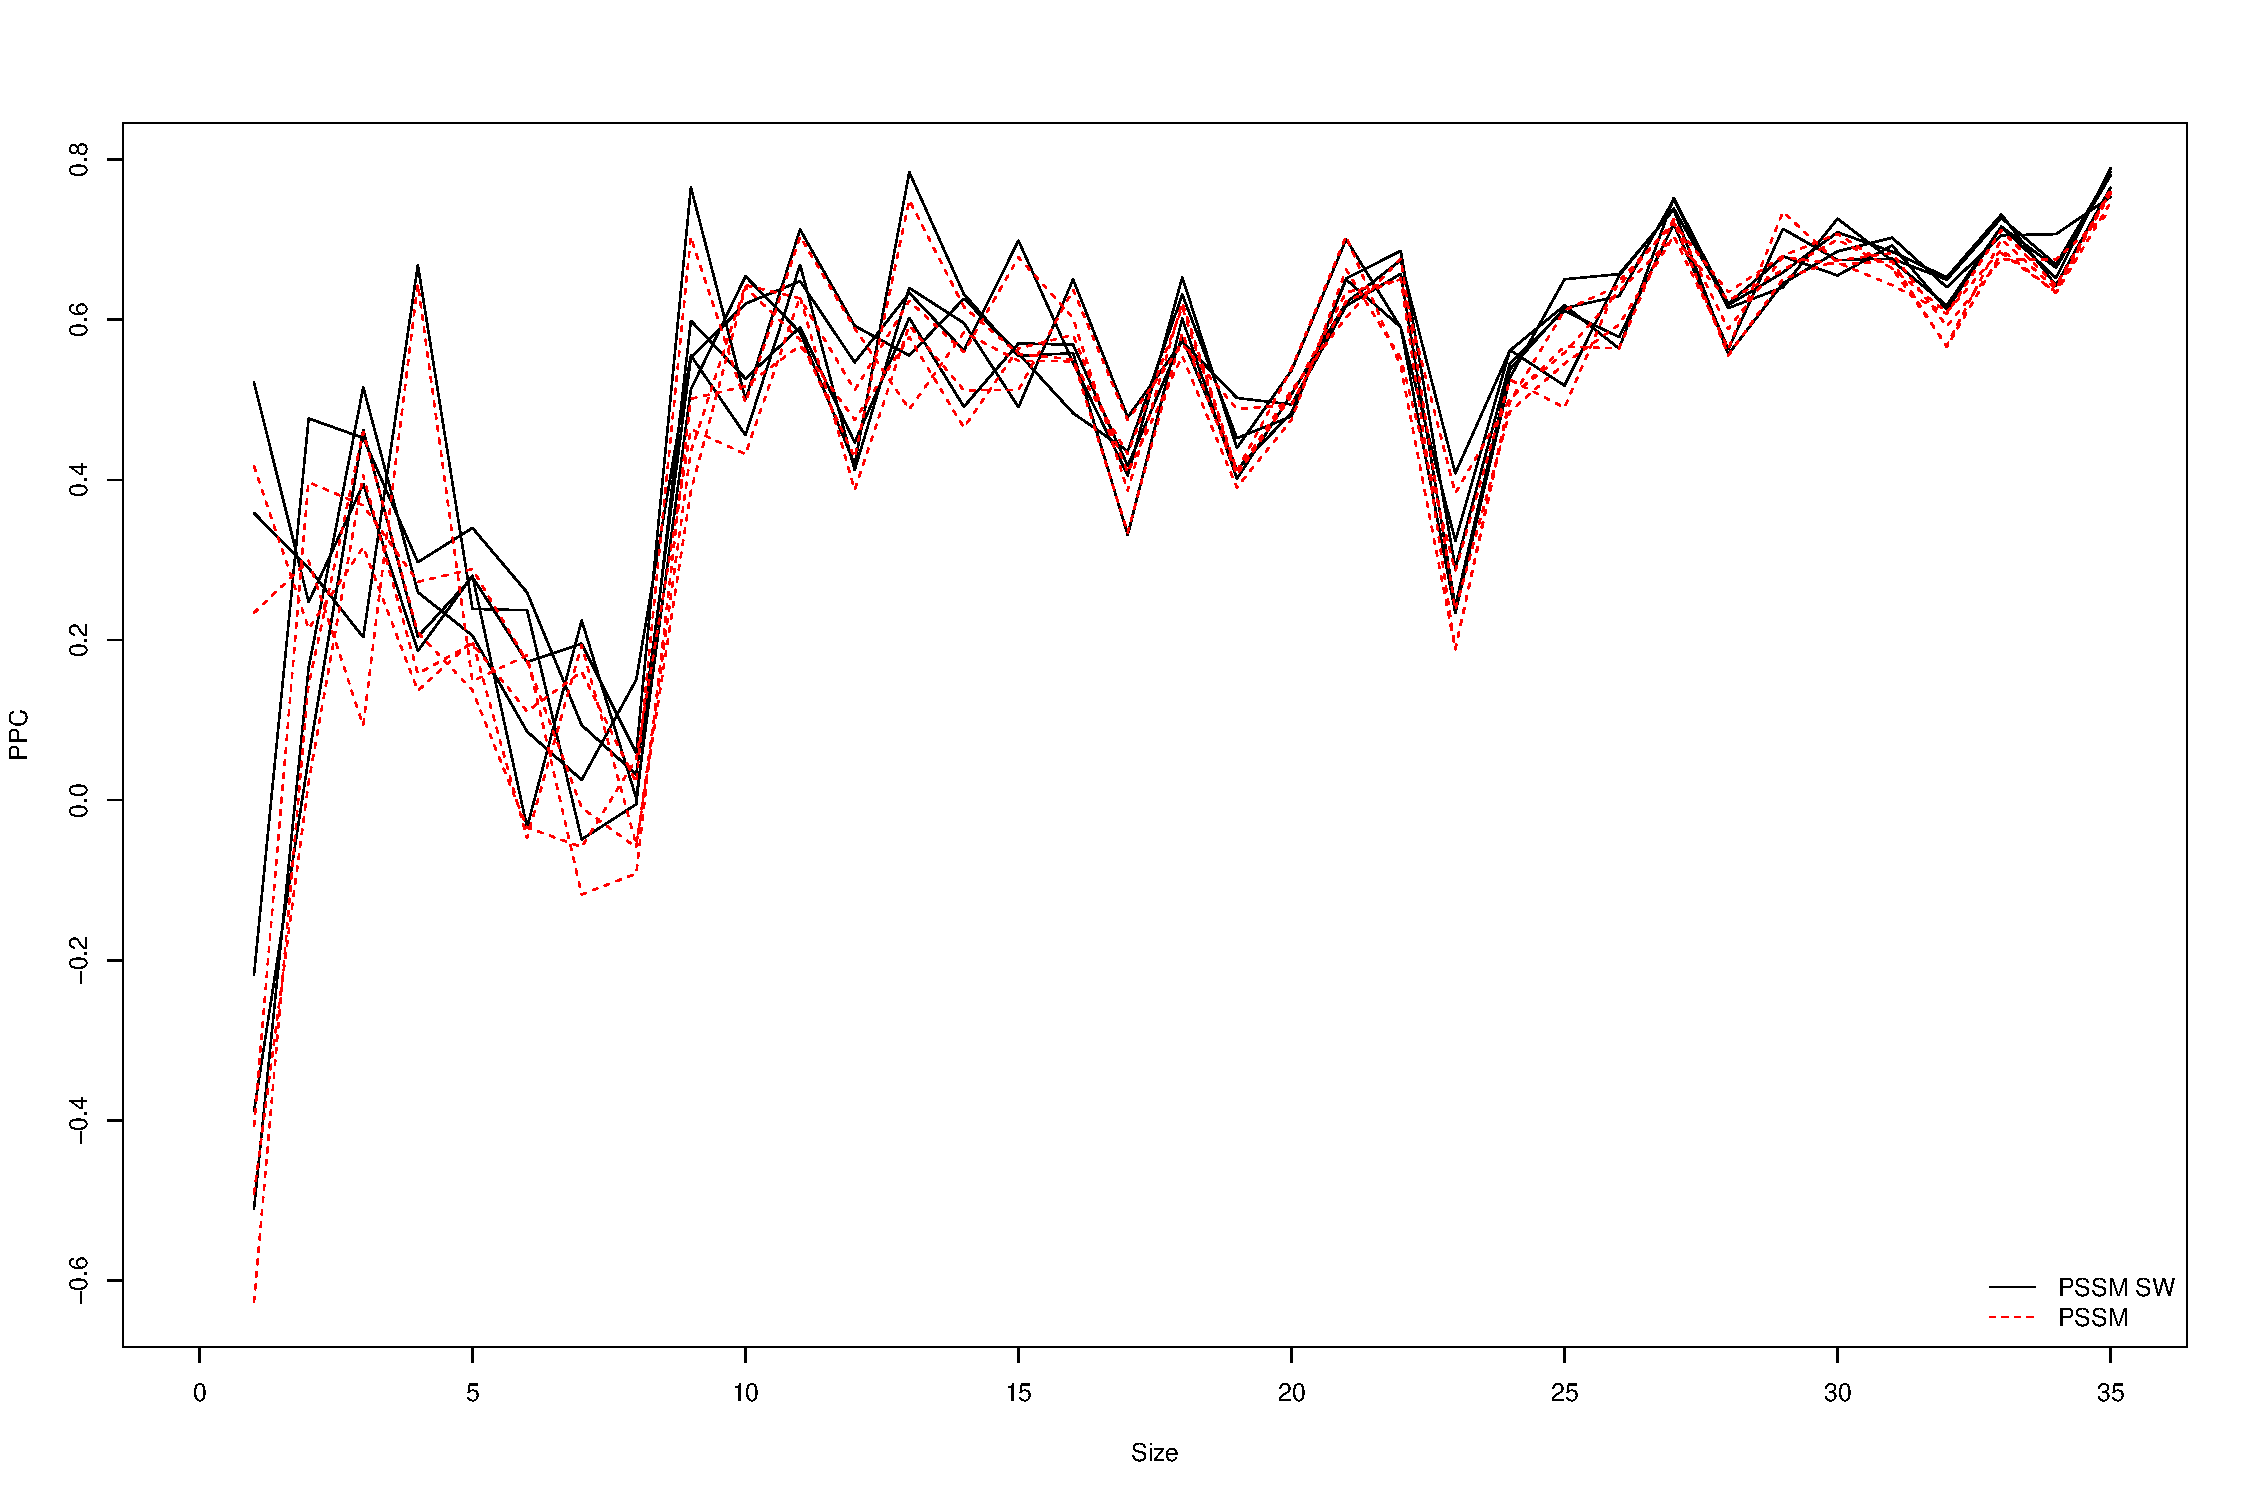
\includegraphics[width=18cm]{fig/pssmLN1.pdf}
\caption{Plot of the average Pearson Correlation Coefficient of the 5 test for the PSSM algorithm on each of the 35 alleles. The alleles are ordered by the number of peptide inside the data, the order is the following:
B5701, A3002, A2301, B4501, B1801, B4002, B4403, B4402, A2902, A2402, B5101, A2403, B5301, B5401, A3001, A2601, B0801, B3501, A6901, B2705, B1501, B5801, B4001, A6801, A3301, A0101, B0702, A6802, A0206, A0203, A0202, A3101, A1101, A0301 and A0201.}\label{fig:pssm1}
\end{center}
\end{figure*}

\begin{figure*}[ht]
\begin{center}
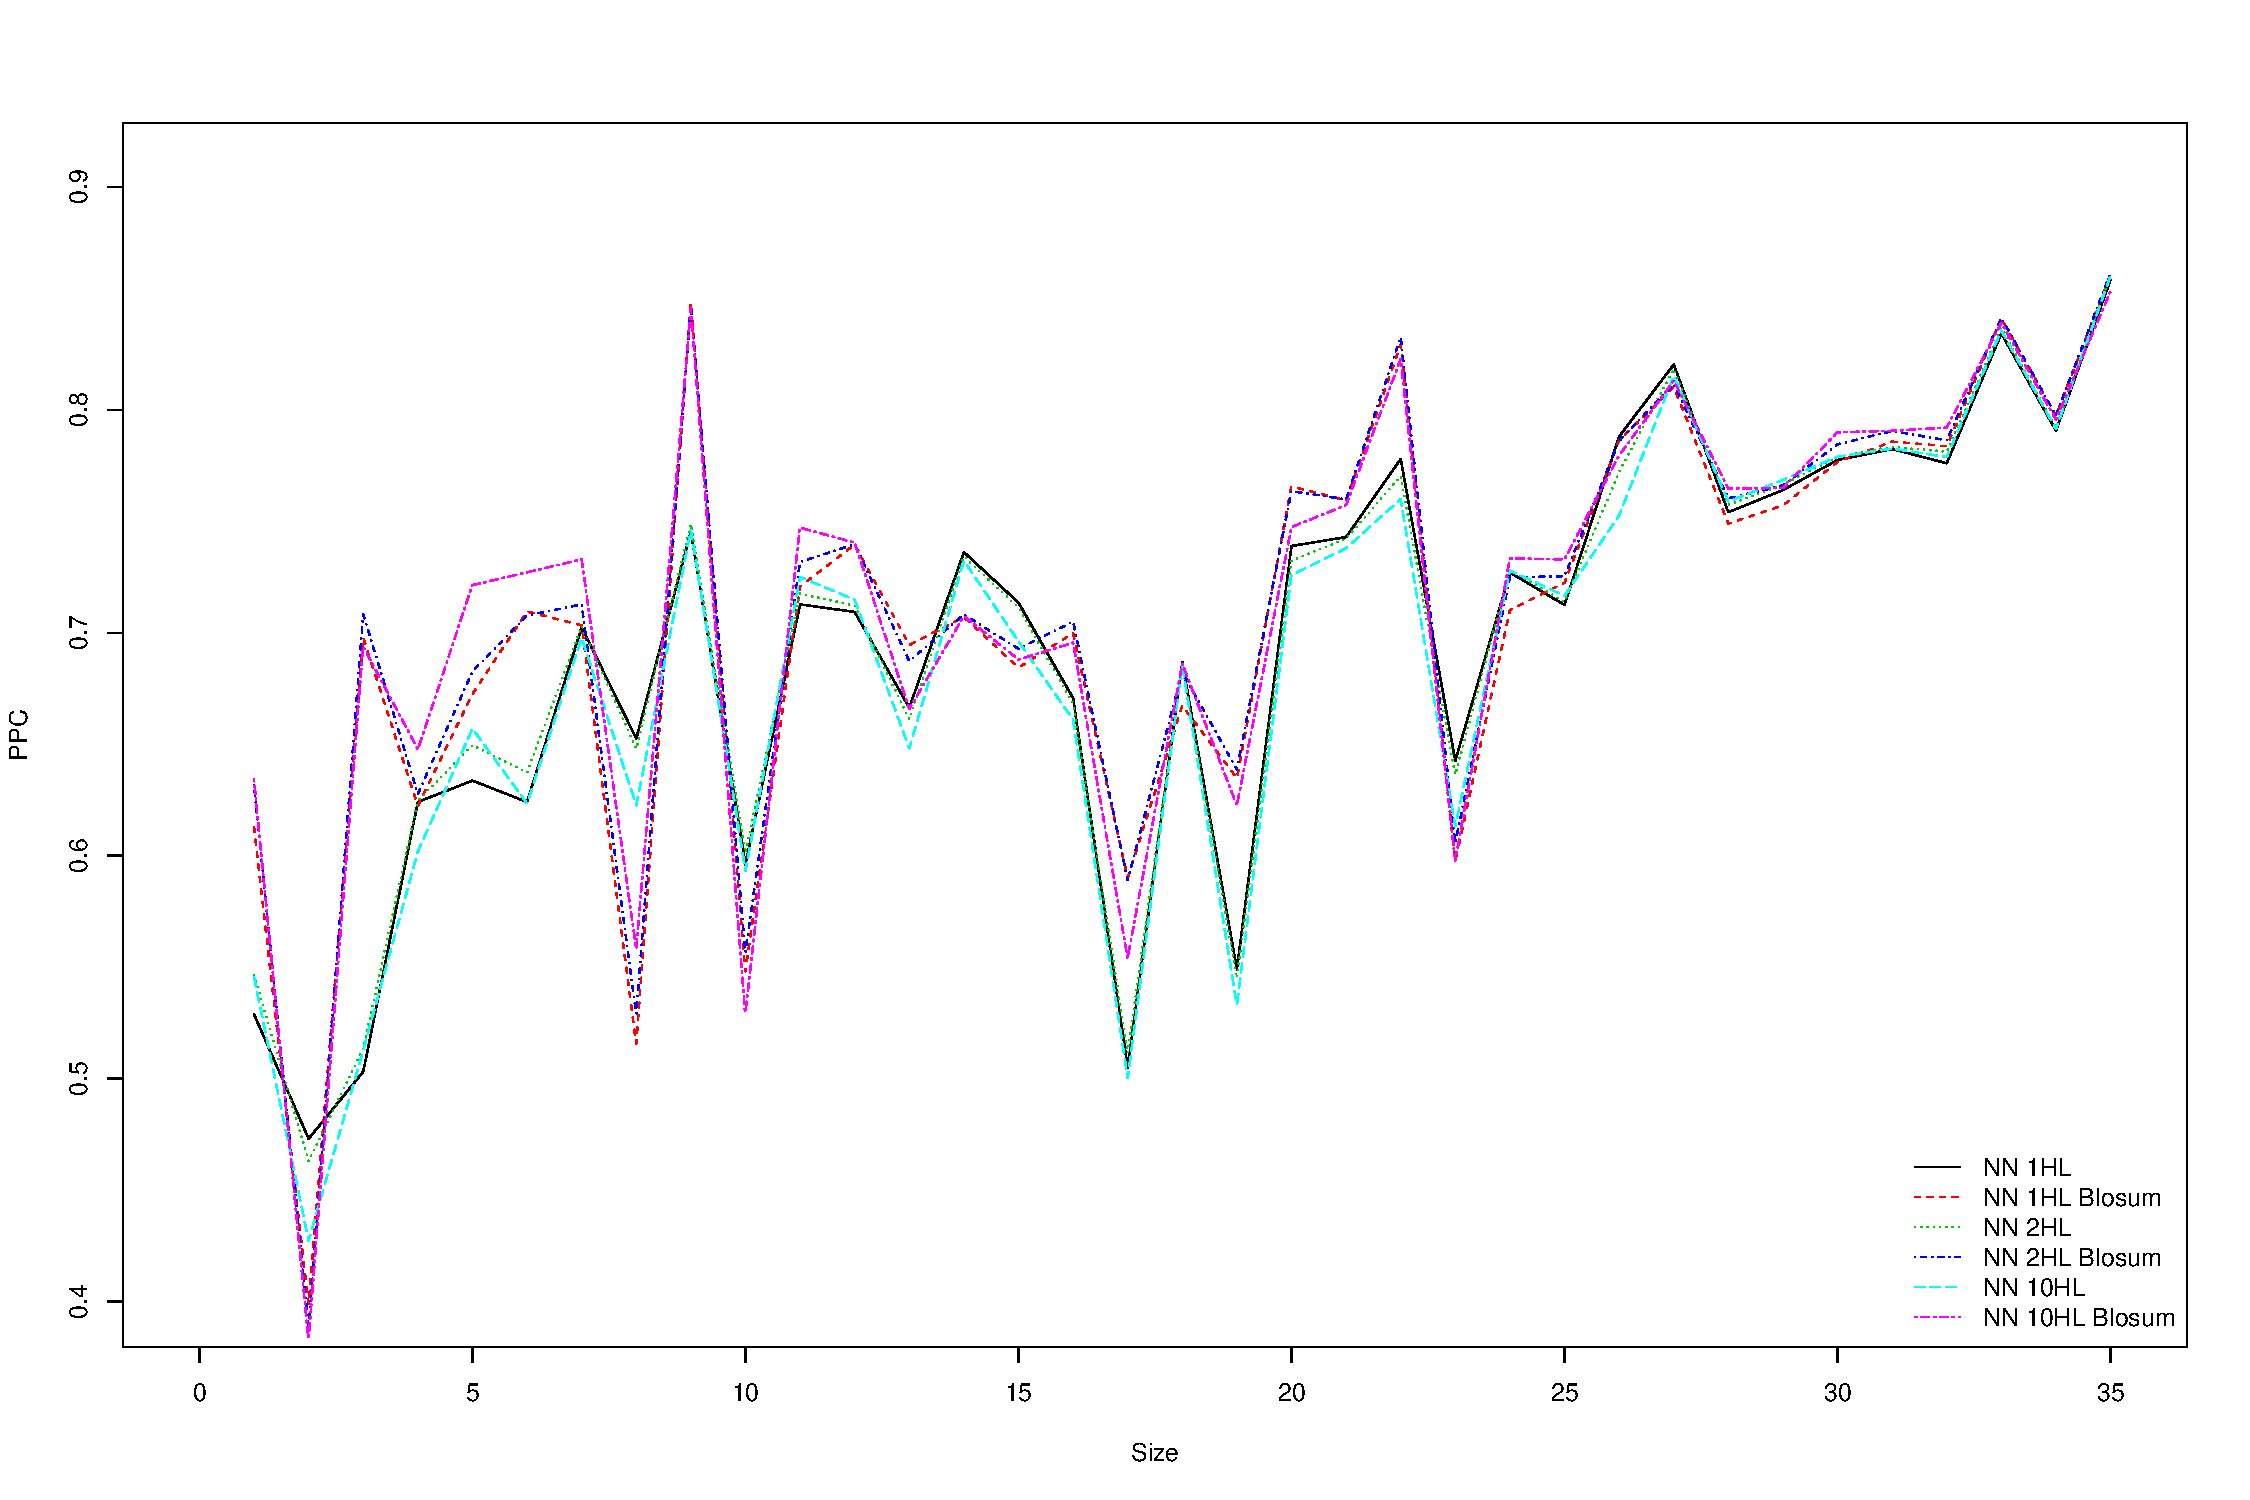
\includegraphics[width=18cm]{fig/annLNzoom.pdf}
\caption{Plot of the average Pearson Correlation Coefficient of the 5 test for the Artificial Neural Network algorithm on each of the 35 alleles. The alleles are ordered by the number of peptide in the dataset. The order is the following:
B5701, A3002, A2301, B4501, B1801, B4002, B4403, B4402, A2902, A2402, B5101, A2403, B5301, B5401, A3001, A2601, B0801, B3501, A6901, B2705, B1501, B5801, B4001, A6801, A3301, A0101, B0702, A6802, A0206, A0203, A0202, A3101, A1101, A0301 and A0201.}\label{fig:ann1}
\end{center}
\end{figure*}

\begin{figure*}[ht]
\begin{center}
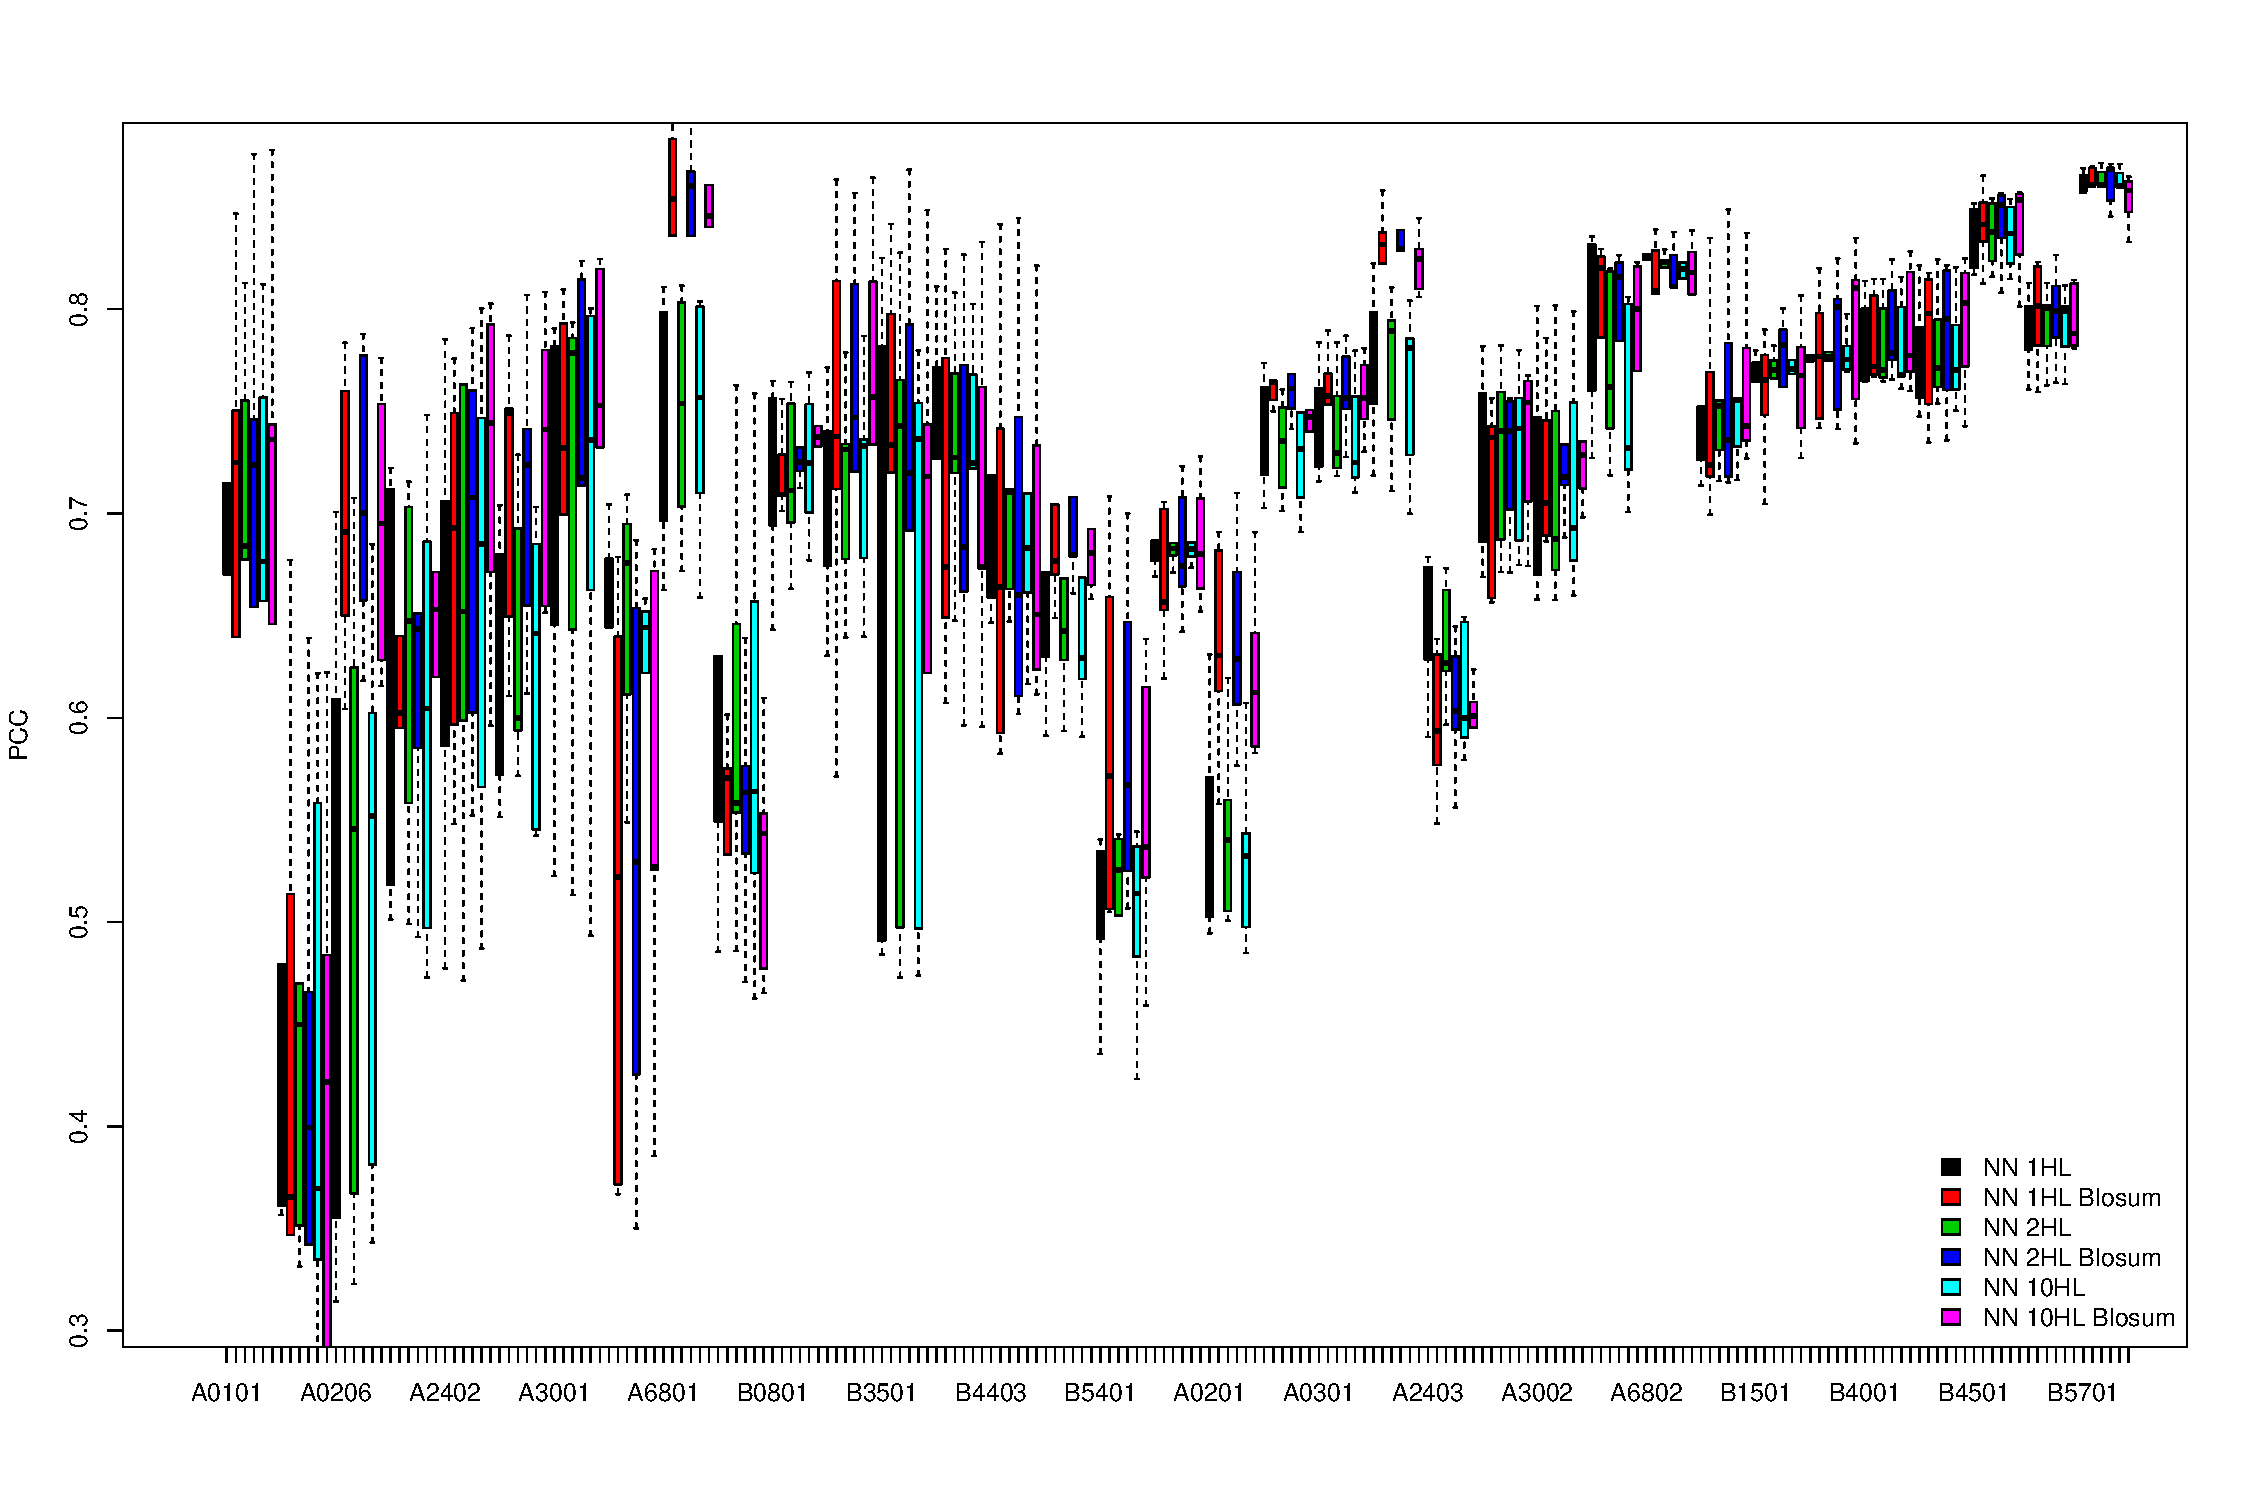
\includegraphics[width=18cm]{fig/annBX1.pdf}
\caption{Boxplot of the Pearson Correlation Coefficient of test with the ANN algorithm on the 35 different alleles. The alleles are ordered by the number of peptide in the dataset. The order in the y axis is the following:
B5701, A3002, A2301, B4501, B1801, B4002, B4403, B4402, A2902, A2402, B5101, A2403, B5301, B5401, A3001, A2601, B0801, B3501, A6901, B2705, B1501, B5801, B4001, A6801, A3301, A0101, B0702, A6802, A0206, A0203, A0202, A3101, A1101, A0301 and A0201.}\label{fig:ann2}
\end{center}
\end{figure*}

PSSM
A Position-specific scoring matrix, also called position weight matrix is a commonly used representation of motifs in biological sequences. It has one row for each symbol in the alphabet (each amino acid, for instance) and one column for each position in the motif. The score is the sum of position-specific scores for each symbol in the substring.



j represents position in the substring, sj is the symbol at position j in the substring and msj,j is the corresponding score in the weight matrix. The weight matrix is constructed using log-odds score



i being the position in the morif and j the amino acid. qj is the background frequency for amno acid j
The information content of a PSSM is an indicator of how different its distribution is from a uniform distribution and is calculated using Shannon's discrete entropy law (the sum part of the equation)



where pi,j is the probability of symbol i in position j.
\subsection*{PSSM} scores can be interpreted as the sum of binding energies for all nucleotides or amino acids (symbols of the substring) aligned with the PSSM and can as such be used to estimate MHC peptide binding affinity.

\subsection*{SVM}
Support vector machines is a set of supervised learning methods used for classification and regression analysis. The standard SVM is non-probabilistic binary linear classifier. It constructs a hyperplane where the seperation is where there is largest distance to the nearest training data point of any class. Nonlinear classification can be achived by  mapping the original space to a higher dimensional feature space and/or select a kernel function to suit the problem. The kernel function plays the role of the dot product in the feature space.

\subsection*{ANN}
We mostly used peptide binding data from class-I MHC molecules (A and B types) as they were most readlily available for us.

\section*{Results}
   % Results



Although quite successful the results of the machine learning methods do not give one much insight into the 'mechanical' workings of the MHC binding.
PSSM weight matrices can also quite accurately describe a sequence motif like MHC class I. In fact their results come quite close to the machine learning methods for the larger datasets. 
Based on results from the three alleles A*0201, A*3001 and B*4001, the ANN's are though performing best overall.
As a pattern recognition tool, ANN with peptide binding data could give some clues for further study on the crystal structure of the MHC proteins.
As stated in the class exercise slides, the ANN's seem to have had a bad reputation. 
It is our guess that the good performance of ANN's in this case is because they are well suited to solve the MHC peptide binding problem. 
Also the correct use and training of the ANN's in terms of overfitting is an helping factor.
By the way in this section we will list the results obtained testing the PSSM, SVM and ANN algorithms on 35 HLA alleles.

\subsection*{PSSM}


C programs from the course were used to estimate MHC binding affinity with PSSM. 
Here a threshold must be used to limit included peptides to the ones that actually bind to the MHC molecule. 
In the machine learning methods non-binding data is also be valuable in the estimation.

All entries from the training data set with binding affinity over 0.426 are feeded into a program. 
This value means that the peptide successfully binds to the MHC molecule. All peptides have the same length.

To prevent overfitting in the creation of the PSSM matrix, we split the data into 5 parts. 4/5 are used in creating the matrix and 1/5 in evaluating it.
Experimental data from the HLA-A*0201 allele is randomly split up in training and evaluation sections, the evaluation section being 1/5 of the training data size (618 peptides vs 2471 peptides in the training set).
For 5 different samplings and using sequence weighting we get a Pearson correlation coefficients of {0.75323,, 0.78415, 0.78009, 0.78896, 0.76480}, the average being 0.774 (see Tab \ref{tab:pssm1} first column).
We also try the smaller set HLA-A*3001. It has a total of 669 experimentally verified peptides.
Using sequence weighting the correlation results are 0.69872, 0.55787, 0.65032, 0.55827 and 0.57044 (see Tab \ref{tab:pssm1} Second Column), an average of 0.607
The corresponding results without using sequence weighting are 0.67775, 0.54853, 0.63731, 0.55026 and 0.56416, with average of 0.596.
From Figure \ref{fig:pssm1} it interesting the case of HLA-B*4001, in which even if there are a considerable number of peptides, the algorithm have poor results (Tab \ref{tab:pssm1} third column). Looking at Table \ref{ftable} is it clear that the little percentage of binding peptides is the cause of so poor performance. 
As seen in Figure \ref{fig:pssm1}, using sequence weighting is gives better results in most cases (of 35 alleles).

Using a small dataset the benefit of using a blosum frequency substitution matrix is greater.
\begin{table*}\scriptsize

\begin{center}

\begin{tabular}{rrr}

\begin{tabular}{rllrrr}
  \hline
 & Param & Allele & Sample & Size & PCC \\ 
  \hline
 & PSSM w/o SW & A0201 &   0 & 618 & 0.74 \\ 
 & PSSM w/o SW & A0201 &   1 & 618 & 0.76 \\ 
 & PSSM w/o SW & A0201 &   2 & 618 & 0.76 \\ 
 & PSSM w/o SW & A0201 &   3 & 618 & 0.76 \\ 
 & PSSM w/o SW & A0201 &   4 & 617 & 0.75 \\ 
\hline
 & PSSM w SW & A0201 &   0 & 618 & 0.75 \\ 
 & PSSM w SW & A0201 &   1 & 618 & 0.78 \\ 
 & PSSM w SW & A0201 &   2 & 618 & 0.78 \\ 
 & PSSM w SW & A0201 &   3 & 618 & 0.79 \\ 
 & PSSM w SW & A0201 &   4 & 617 & 0.76 \\ 
   \hline
\end{tabular}

\begin{tabular}{rllrrr}
  \hline
 & Param & Allele & Sample & Size & PCC \\ 
  \hline
   & PSSM & A3001 &   0 & 134 & 0.68 \\ 
   & PSSM & A3001 &   1 & 134 & 0.55 \\ 
   & PSSM & A3001 &   2 & 134 & 0.64 \\ 
   & PSSM & A3001 &   3 & 134 & 0.55 \\ 
   & PSSM & A3001 &   4 & 133 & 0.56 \\ 
  \hline
   & PSSM SW & A3001 &   0 & 134 & 0.70 \\ 
   & PSSM SW & A3001 &   1 & 134 & 0.56 \\ 
   & PSSM SW & A3001 &   2 & 134 & 0.65 \\ 
   & PSSM SW & A3001 &   3 & 134 & 0.56 \\ 
   & PSSM SW & A3001 &   4 & 133 & 0.57 \\ 
   \hline
\end{tabular}

\begin{tabular}{rllrrr}
  \hline
 & Param & Allele & Sample & Size & PCC \\ 
  \hline
   & PSSM & B4001 &   0 & 216 & 0.19 \\ 
   & PSSM & B4001 &   1 & 216 & 0.24 \\ 
   & PSSM & B4001 &   2 & 216 & 0.19 \\ 
   & PSSM & B4001 &   3 & 215 & 0.38 \\ 
   & PSSM & B4001 &   4 & 215 & 0.29 \\ 
\hline
   & PSSM SW & B4001 &   0 & 216 & 0.23 \\ 
   & PSSM SW & B4001 &   1 & 216 & 0.29 \\ 
   & PSSM SW & B4001 &   2 & 216 & 0.24 \\ 
   & PSSM SW & B4001 &   3 & 215 & 0.41 \\ 
   & PSSM SW & B4001 &   4 & 215 & 0.32 \\ 
   \hline
\end{tabular}

\end{tabular}
\end{center}
\caption{Summary of the PSSM results for three most significant alleles, A0201, A3001 and B4001. Looking also at the data in Tab \ref{ftable} we can see that even if B4001 have a great number of peptides in the dataset, only the 4\% is binding. This is translate in the results with a really bad estimation of the binding}\label{tab:pssm1}
\end{table*}

\subsection*{SVM}
In this investigation version 3.6.3 of the java based Weka software is used for SVM calculations.
The data has to be prepared for input into the Weka program.
The number of amino acids is 20 and the length of the peptide is 9 so each peptide is changed to a vector of length 20*9. 
Three encoding schemes are used, blosum50, sparse and z-score. 
In the case of the blosum encoding scheme, each of the 9 sections of length 20 simply contain the data from each row in blosum matrix corresponding to the amino acid in question.
The sparse encoding uses the identity substitution matrix. 
The z-score encoding is a condensed manner to represent each amino acid, only 5 values are used to encode each amino acid based on on their properties. 
These properties were deduced from measured data using thin-layer chromatography and nuclear magnetic resonance and some calculated variables 
such as side chain charge, hydrogen bond donor and acceptor properties, log P and molecular weight. 
Each row in the input matrix has therefore length of 5*20+1 (the one being the measured affinity value)
The same data as from the PSSM section is used for comparison. For the HLA-A*0201 dataset and sparse encoding we get the results displayed in the first line of table \ref{tab:svm1}.

For the A*0201 allele, the SMO classifier (Table \ref{tab:svm1} second line) using sparse encoded data with polynomial kernel of first degree gives slightly better results than the PSSM. Raising the degree of the kernel to 2 does not improve the results.

Using the blosum matrix with a kernel of degree of 1 gives almost the same results as a sparse encoding (Table \ref{tab:svm1} the 3$^{rd}$ line). Polynomial kernel of degree 2 has considerably worse performance for the blosum encoded data (see Tab \ref{tab:svm1} line 4 ). Also the z-score encoded data with polynomial kernel of degree 1 (Tab \ref{tab:svm1} line 5) does not give better results.
Trying the same tests with a smaller dataset, the HLA-A*3001 (Tab \ref{tab:svm1} in the 6$^{th}$ line), we notice that blosum encoded data slightly raises the prediction performance (Tab \ref{tab:svm1} in the 7$^{th}$ line).

\begin{table}[ht]\scriptsize
\begin{center}
\begin{tabular}{rllrrr}
  \hline
 & Param & Allele & Size & PCC & MAE \\ 
  \hline
 & SVM Pol. 1$^{st}$ d + Sparse & A0201 &   618 & 0.78 & 0.1524 \\ 
 & SVM Pol. 2$^{st}$ degree & A0201 &   618 & 0.756 & 0.1535 \\ 
 & SVM Pol. 1$^{st}$ d + Blosum & A0201 &   618 & 0.7789 & 0.1533 \\ 
 & SVM Pol. 2$^{nd}$ degree & A0201 &   618 & 0.6692 & 0.2047 \\ 
 & SVM Pol. 1$^{st}$ d + z-score & A0201 &   618 & 0.6888 & 0.1802 \\ 
 & SVM Sparse & A3001 &   134 & 0.7412 & 0.1008 \\ 
 & SVM Pol. 1$^{nd}$ d + Blosum & A3001 &   134 & 0.7671 & 0.0945 \\ 
 & SVM Pol. 1$^{nd}$ d + Sparse & B4001 &   216 & 0.4876 & 0.0373 \\ 
 & SVM Pol. 1$^{nd}$ d + Blosum & B4001 &   216 & 0.4456 & 0.0387 \\ 
 & SVM Pol. 1$^{nd}$ d + Zscore & B4001 &   216 & 0.2397 & 0.0400 \\ 
   \hline
\end{tabular}
\end{center}
\caption{Result table for SVM with various kernel and various encoding schema. The three alleles A0201, A3001 and B4001 were considered.}\label{tab:svm1}
\end{table}

\begin{table*}[hb]\scriptsize
\begin{center}
\begin{tabular}{rrr}

\begin{tabular}{rllrrr}
  \hline
 & Param & Allele & Sample & Size & PCC \\ 
  \hline
   & NN 10HL & A0201 &   0 & 618 & 0.84 \\ 
   & NN 10HL & A0201 &   1 & 618 & 0.87 \\ 
   & NN 10HL & A0201 &   2 & 618 & 0.86 \\ 
   & NN 10HL & A0201 &   3 & 618 & 0.86 \\ 
   & NN 10HL & A0201 &   4 & 617 & 0.87 \\ 
   \hline
   & NN 10HL Blosum & A0201 &   0 & 618 & 0.83 \\ 
   & NN 10HL Blosum & A0201 &   1 & 618 & 0.86 \\ 
   & NN 10HL Blosum & A0201 &   2 & 618 & 0.85 \\ 
   & NN 10HL Blosum & A0201 &   3 & 618 & 0.86 \\ 
   & NN 10HL Blosum & A0201 &   4 & 617 & 0.86 \\ 
   \hline
   & NN 1HL & A0201 &   0 & 618 & 0.84 \\ 
   & NN 1HL & A0201 &   1 & 618 & 0.87 \\ 
   & NN 1HL & A0201 &   2 & 618 & 0.86 \\ 
   & NN 1HL & A0201 &   3 & 618 & 0.86 \\ 
   & NN 1HL & A0201 &   4 & 617 & 0.87 \\ 
   \hline
   & NN 1HL Blosum & A0201 &   0 & 618 & 0.84 \\ 
   & NN 1HL Blosum & A0201 &   1 & 618 & 0.87 \\ 
   & NN 1HL Blosum & A0201 &   2 & 618 & 0.86 \\ 
   & NN 1HL Blosum & A0201 &   3 & 618 & 0.86 \\ 
   & NN 1HL Blosum & A0201 &   4 & 617 & 0.87 \\ 
   \hline
   & NN 2HL & A0201 &   0 & 618 & 0.84 \\ 
   & NN 2HL & A0201 &   1 & 618 & 0.87 \\ 
   & NN 2HL & A0201 &   2 & 618 & 0.86 \\ 
   & NN 2HL & A0201 &   3 & 618 & 0.86 \\ 
   & NN 2HL & A0201 &   4 & 617 & 0.87 \\ 
   \hline
   & NN 2HL Blosum & A0201 &   0 & 618 & 0.85 \\ 
   & NN 2HL Blosum & A0201 &   1 & 618 & 0.87 \\ 
   & NN 2HL Blosum & A0201 &   2 & 618 & 0.85 \\ 
   & NN 2HL Blosum & A0201 &   3 & 618 & 0.87 \\ 
   & NN 2HL Blosum & A0201 &   4 & 617 & 0.87 \\ 
   \hline
\end{tabular}


\begin{tabular}{rllrrr}
  \hline
 & Param & Allele & Sample & Size & PCC \\ 
  \hline
   & NN 10HL & A3001 &   0 & 134 & 0.81 \\ 
   & NN 10HL & A3001 &   1 & 134 & 0.66 \\ 
   & NN 10HL & A3001 &   2 & 134 & 0.80 \\ 
   & NN 10HL & A3001 &   3 & 134 & 0.67 \\ 
   & NN 10HL & A3001 &   4 & 133 & 0.71 \\ 
\hline
   & NN 10HL Blosum & A3001 &   0 & 134 & 0.82 \\ 
   & NN 10HL Blosum & A3001 &   1 & 134 & 0.65 \\ 
   & NN 10HL Blosum & A3001 &   2 & 134 & 0.78 \\ 
   & NN 10HL Blosum & A3001 &   3 & 134 & 0.68 \\ 
   & NN 10HL Blosum & A3001 &   4 & 133 & 0.62 \\ 
\hline
   & NN 1HL & A3001 &   0 & 134 & 0.83 \\ 
   & NN 1HL & A3001 &   1 & 134 & 0.66 \\ 
   & NN 1HL & A3001 &   2 & 134 & 0.81 \\ 
   & NN 1HL & A3001 &   3 & 134 & 0.67 \\ 
   & NN 1HL & A3001 &   4 & 133 & 0.72 \\ 
\hline
   & NN 1HL Blosum & A3001 &   0 & 134 & 0.84 \\ 
   & NN 1HL Blosum & A3001 &   1 & 134 & 0.66 \\ 
   & NN 1HL Blosum & A3001 &   2 & 134 & 0.80 \\ 
   & NN 1HL Blosum & A3001 &   3 & 134 & 0.67 \\ 
   & NN 1HL Blosum & A3001 &   4 & 133 & 0.59 \\ 
\hline
   & NN 2HL & A3001 &   0 & 134 & 0.82 \\ 
   & NN 2HL & A3001 &   1 & 134 & 0.66 \\ 
   & NN 2HL & A3001 &   2 & 134 & 0.81 \\ 
   & NN 2HL & A3001 &   3 & 134 & 0.67 \\ 
   & NN 2HL & A3001 &   4 & 133 & 0.71 \\ 
\hline
   & NN 2HL Blosum & A3001 &   0 & 134 & 0.84 \\ 
   & NN 2HL Blosum & A3001 &   1 & 134 & 0.66 \\ 
   & NN 2HL Blosum & A3001 &   2 & 134 & 0.80 \\ 
   & NN 2HL Blosum & A3001 &   3 & 134 & 0.68 \\ 
   & NN 2HL Blosum & A3001 &   4 & 133 & 0.60 \\ 
   \hline
\end{tabular}

\begin{tabular}{rllrrr}
  \hline
 & Param & Allele & Sample & Size & PCC \\ 
  \hline
   & NN 10HL & B4001 &   0 & 216 & 0.58 \\ 
   & NN 10HL & B4001 &   1 & 216 & 0.65 \\ 
   & NN 10HL & B4001 &   2 & 216 & 0.60 \\ 
   & NN 10HL & B4001 &   3 & 215 & 0.59 \\ 
   & NN 10HL & B4001 &   4 & 215 & 0.65 \\ 
\hline
   & NN 10HL Blosum & B4001 &   0 & 216 & 0.61 \\ 
   & NN 10HL Blosum & B4001 &   1 & 216 & 0.62 \\ 
   & NN 10HL Blosum & B4001 &   2 & 216 & 0.56 \\ 
   & NN 10HL Blosum & B4001 &   3 & 215 & 0.60 \\ 
   & NN 10HL Blosum & B4001 &   4 & 215 & 0.60 \\ 
\hline
   & NN 1HL & B4001 &   0 & 216 & 0.59 \\ 
   & NN 1HL & B4001 &   1 & 216 & 0.67 \\ 
   & NN 1HL & B4001 &   2 & 216 & 0.64 \\ 
   & NN 1HL & B4001 &   3 & 215 & 0.63 \\ 
   & NN 1HL & B4001 &   4 & 215 & 0.68 \\ 
\hline
   & NN 1HL Blosum & B4001 &   0 & 216 & 0.64 \\ 
   & NN 1HL Blosum & B4001 &   1 & 216 & 0.59 \\ 
   & NN 1HL Blosum & B4001 &   2 & 216 & 0.55 \\ 
   & NN 1HL Blosum & B4001 &   3 & 215 & 0.63 \\ 
   & NN 1HL Blosum & B4001 &   4 & 215 & 0.58 \\ 
\hline
   & NN 2HL & B4001 &   0 & 216 & 0.60 \\ 
   & NN 2HL & B4001 &   1 & 216 & 0.66 \\ 
   & NN 2HL & B4001 &   2 & 216 & 0.63 \\ 
   & NN 2HL & B4001 &   3 & 215 & 0.62 \\ 
   & NN 2HL & B4001 &   4 & 215 & 0.67 \\ 
\hline
   & NN 2HL Blosum & B4001 &   0 & 216 & 0.64 \\ 
   & NN 2HL Blosum & B4001 &   1 & 216 & 0.60 \\ 
   & NN 2HL Blosum & B4001 &   2 & 216 & 0.56 \\ 
   & NN 2HL Blosum & B4001 &   3 & 215 & 0.63 \\ 
   & NN 2HL Blosum & B4001 &   4 & 215 & 0.59 \\ 
   \hline
\end{tabular}
\end{tabular}
\end{center}

\caption{Summary of the Artificial Neural Network algorithm results for three alleles: A0201, A3001 and B4001. Referring to the data in Tab \ref{ftable} we can see that even if B4001 have a great number of peptides in the dataset, only the 4\% is binding. By the way the performance of the ANN algorithm it is still better compared to the other algorithms in this article.}\label{tab:nn1}

\end{table*}

\subsection*{ANN}



The \textit{nnbackprop} and the \textit{nnforward} algorithms from the course were used in order to estimate the MHC binding affinity.
In the figure \ref{fig:ann1} and figure \ref{fig:ann2} are summarized the results for all the 35 alleles, ordered by the number of peptides in each sample.
The back propagation algorithm was tested with 10, 2 and 1 hidden layers, on data with and without Blosum encoding. The total combination of the given options amount then to 6 different configuration for each allele.

In table \ref{tab:nn1} are listed the results for each separate test for the three alleles A0201, A3001 and B4001.
The average PCC for A0201 is 0.86, A3001 0.72 and B4001 had PCC average of 0.62.
Regardless the relative option of the algorithm ANN is working much better then PSSM and SVM. We can note in figure \ref{fig:ann2} that in few cases the use of Blosum encoding is stand out respect the sparse encoding. But generally the two encodings performs equally, especially with a larger number of peptide bindings data.
Another interesting fact is that in table \ref{tab:nn1} we can see that artificial neural network somehow is less effected by the low percentage of binding peptides in the dataset (Tab \ref{tab:nn1}, HLA-B*4001 third column).
As general observation is apparent that with the increasing of the size of the sample, the variation in the results narrows. 






C programs from the course were used to estimate MHC binding affinity with PSSM. 
Here a threshold must be used to limit included peptides to the ones that actually bind to the MHC molecule. 
In the machine learing methods non-binding data is also be valuable in the estimation.


\section*{Discussion}
   % Discussion



\section*{Conclusion}
   %Conclusion


%% Make a new page if you want the bib in a new page
\newpage





%\bibliographystyle{natbib}
%\bibliographystyle{achemnat}
%\bibliographystyle{plainnat}
%\bibliographystyle{abbrv}
%\bibliographystyle{bioinformatics}

\bibliographystyle{abbrv}

\bibliography{algo_main}


\end{application}
\end{document}
